
\documentclass{beamer}
\usepackage{beamerthemeBoadilla}


\usepackage[utf8]{inputenc}
\usepackage[portuguese]{babel}
\usepackage{lmodern}
\usepackage[T1]{fontenc}
\usepackage{graphicx}
\usepackage{url}
\usepackage{xspace}
\usepackage{amssymb}
\usepackage{amsmath}
\usepackage{amsfonts}
\usepackage{amsthm}
\renewcommand\sfdefault{phv}
\renewcommand\familydefault{\sfdefault}
%%%%%%%%%%
\usepackage{xcolor}
\usepackage{listings}
\newcommand{\blue}[1]{\textcolor{blue}{#1}}
\newcommand{\red}[1]{\textcolor{red}{#1}}
\definecolor{light-gray}{gray}{0.95}
\lstset{
language=C,
keywordstyle=\color{blue}\textbf,
backgroundcolor=\color{light-gray},
commentstyle=\color{orange},
basicstyle=\ttfamily\small,breaklines=true,
          showspaces=false,
          showstringspaces=false,
          xleftmargin=20pt}

%%%%%%%%%%


\title[ECT2303 - Funções Recursivas\;\;\;\;\; \insertpagenumber]
{ECT2303 - Linguagem de Programação \\ Funções Recursivas}
		
\author[]{Carlos Olarte. 
}

\institute{
}

%\date{06 de agosto de 2015}

\setbeamertemplate{headline}[tree]
{
}

\begin{document} 

\frame{\titlepage}

\begin{frame}[fragile]{Motivação}
Considere as seguintes funções:
\begin{itemize}
 \item $\blue{n!} = 
 \left\{ \begin{array}{lll}
 1 & \quad& \mbox{se }n=0\\
 n \times \red{(n-1)!} & &\mbox{se }n > 0
 \end{array}
 \right.$
 \item $\blue{pow(a,n)} = 
 \left\{ \begin{array}{lll}
 1 & \quad& \mbox{se }n=0\\
 a \times \red{pow(a,n-1)} & &\mbox{se }n > 0
 \end{array}
 \right.$
 \item $\blue{fib(n)} = 
 \left\{ \begin{array}{lll}
 1 & \quad& \mbox{se } 1 \leq n \leq 2\\
 \red{fib(n-1) + fib(n-2)} & &\mbox{se }n > 2
 \end{array}
 \right.$
\end{itemize}

\begin{block}{}
O que elas têm em comum ? 
\end{block}

\end{frame}

\begin{frame}[fragile]{Objetivo da Aula}

\begin{itemize}
 \item Entender o mecanismo de \blue{recursividade} nas linguagens de programação. 
 \item Utilizar o conceito de recursividade para definir funções. 

\end{itemize}


\end{frame}


\begin{frame}[fragile]{Definições}
\begin{block}{}
\begin{itemize}
 \item Uma função \blue{recursiva} é uma função que se refere a \red{si própria}. 
 \item Utilizamos a própria função que estamos a definir na sua definição.
 \end{itemize}
\end{block}

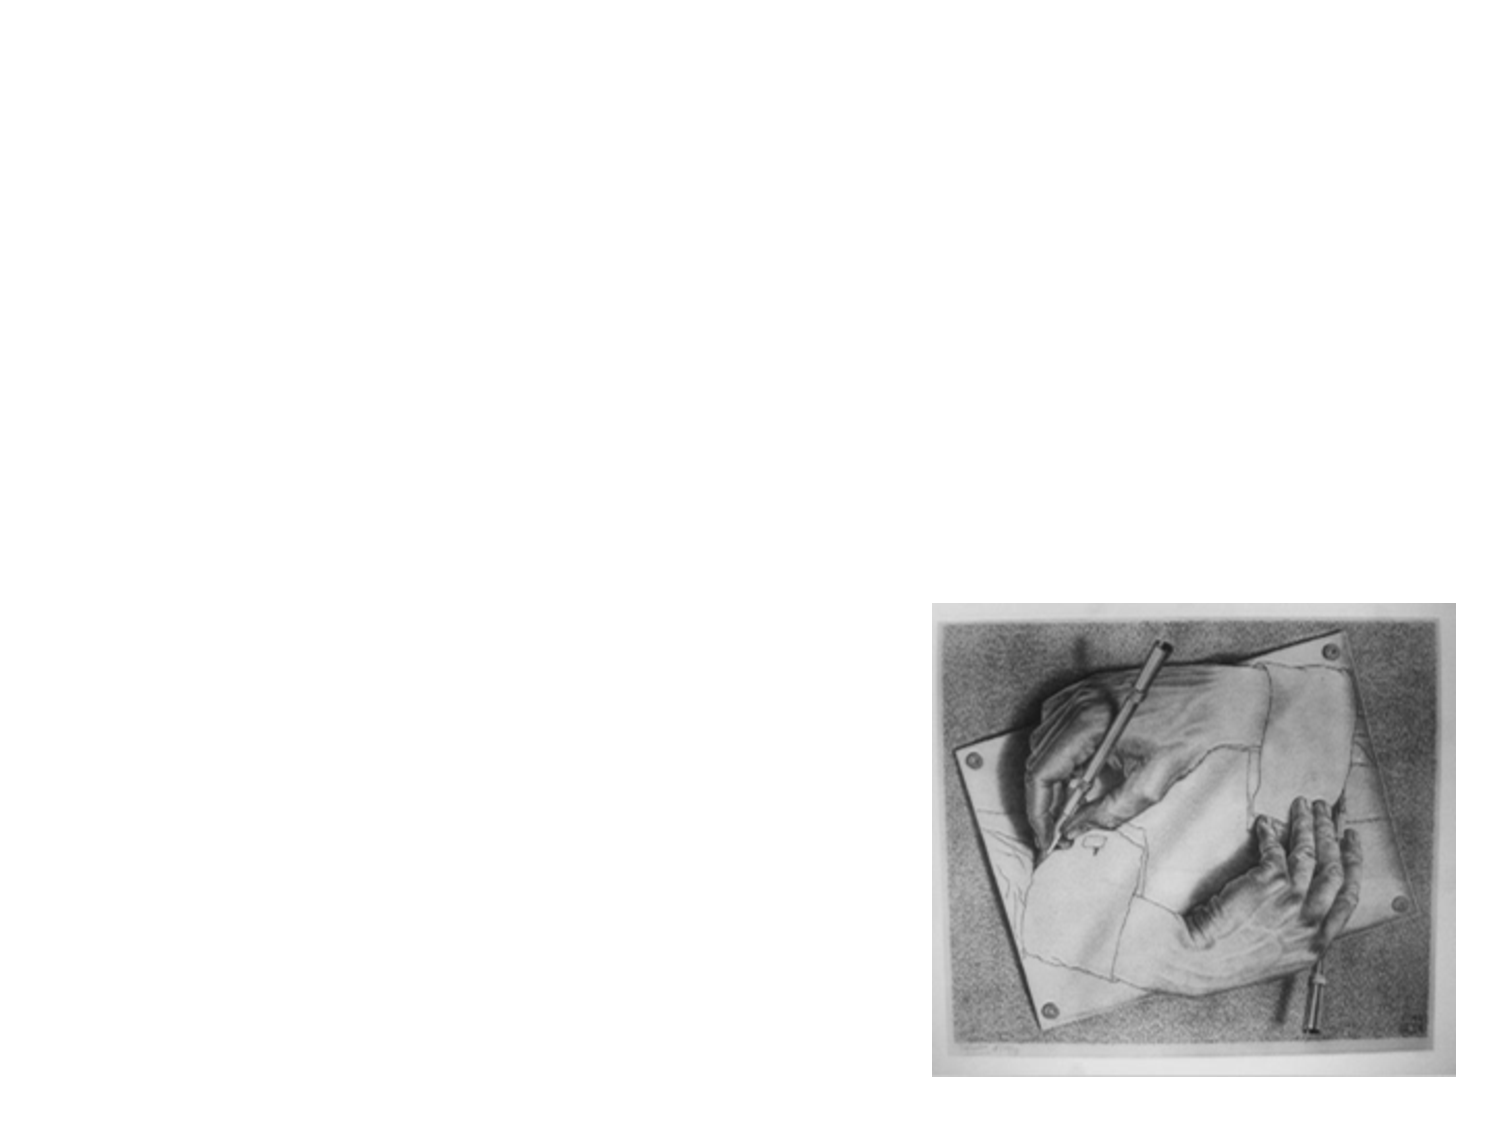
\includegraphics[scale=0.5]{img/escher}
\qquad

\includegraphics[scale=0.4]{img/rec}
\end{frame}


\begin{frame}[fragile]{Funções Recursivas}
\blue{Ideia Geral}:
\begin{itemize}
 \item \red{Caso Base}: o resultado  é conhecido (não precisamos calcula-o).
 \item \red{Caso Recursivo}: para resolver um problema de tamanho $N$, precisamos de uma solução a um problema de tamanho $M<N$ (\blue{subproblemas} do problema inicial). 
\end{itemize}

\[\blue{n!} = 
 \left\{ \begin{array}{lll}
 1 & \quad& \mbox{se }n=0 \ (\mbox{\blue{caso base}})\\
 n \times \red{(n-1)!} & &\mbox{se }n > 0 \ (\mbox{\blue{caso recursivo}})
 \end{array}
 \right.\]
\end{frame}


\begin{frame}[fragile]{Exemplo 1}
\framesubtitle{Execução de funções recursivas}
Versão não recursiva
\begin{lstlisting}
int fatorial (int num){ 
 int prod = 1;
 int i;
 for(i=n;i>=1;i--)
   prod *= i;

 return prod;
}
\end{lstlisting}

Versão recursiva
\begin{lstlisting}
int fatorial (int num){ 
  if (num == 0) 
    return 1;  
  else 
    return num * fatorial (num-1);
}
\end{lstlisting}


\end{frame}


\begin{frame}[fragile]{Exemplo 2: Sequências geradas recursivamente}

1, 1, 2, 3, 5, 8 ... 
\ \\ \ \\
$\blue{fib(n)} = 
 \left\{ \begin{array}{lll}
 1 & \quad& \mbox{se } 1 \leq n \leq 2\\
 \red{fib(n-1) + fib(n-2)} & &\mbox{se }n > 2
 \end{array}
 \right.$
 
\begin{lstlisting}
int fib( int n ){
  if( n <= 2) 
    return 1;
  else
    return fib(n-1) + fib(n-2);
}
\end{lstlisting}


\end{frame}


\begin{frame}[fragile]{Funções Recursivas}
\begin{itemize} 
 \item Em geral, a todo procedimento recursivo corresponde um outro não recursivo (iterativo).
 \end{itemize}
\blue{Vantagens da recursão}:
 \begin{itemize}
  \item algoritmos mais concisos;
  \item simplifica a solução de alguns problemas;
  \item facilidade de implementação e compreensão;
  \item estratégia \blue{divisão e conquista}. 
 \end{itemize}



\end{frame}


\begin{frame}[fragile]{Função Ackermann}
\[
A(m,n) = \left\{ 
\begin{array}{lll}
n+1 & \quad& \mbox{se } m=0 \\
A(m-1,1) & \quad& \mbox{se } m>0 \mbox{ e } n=0 \\
A(m-1, A(m,n-1)) & \quad& \mbox{se } m,n> 0 \\
\end{array}
\right.
\]
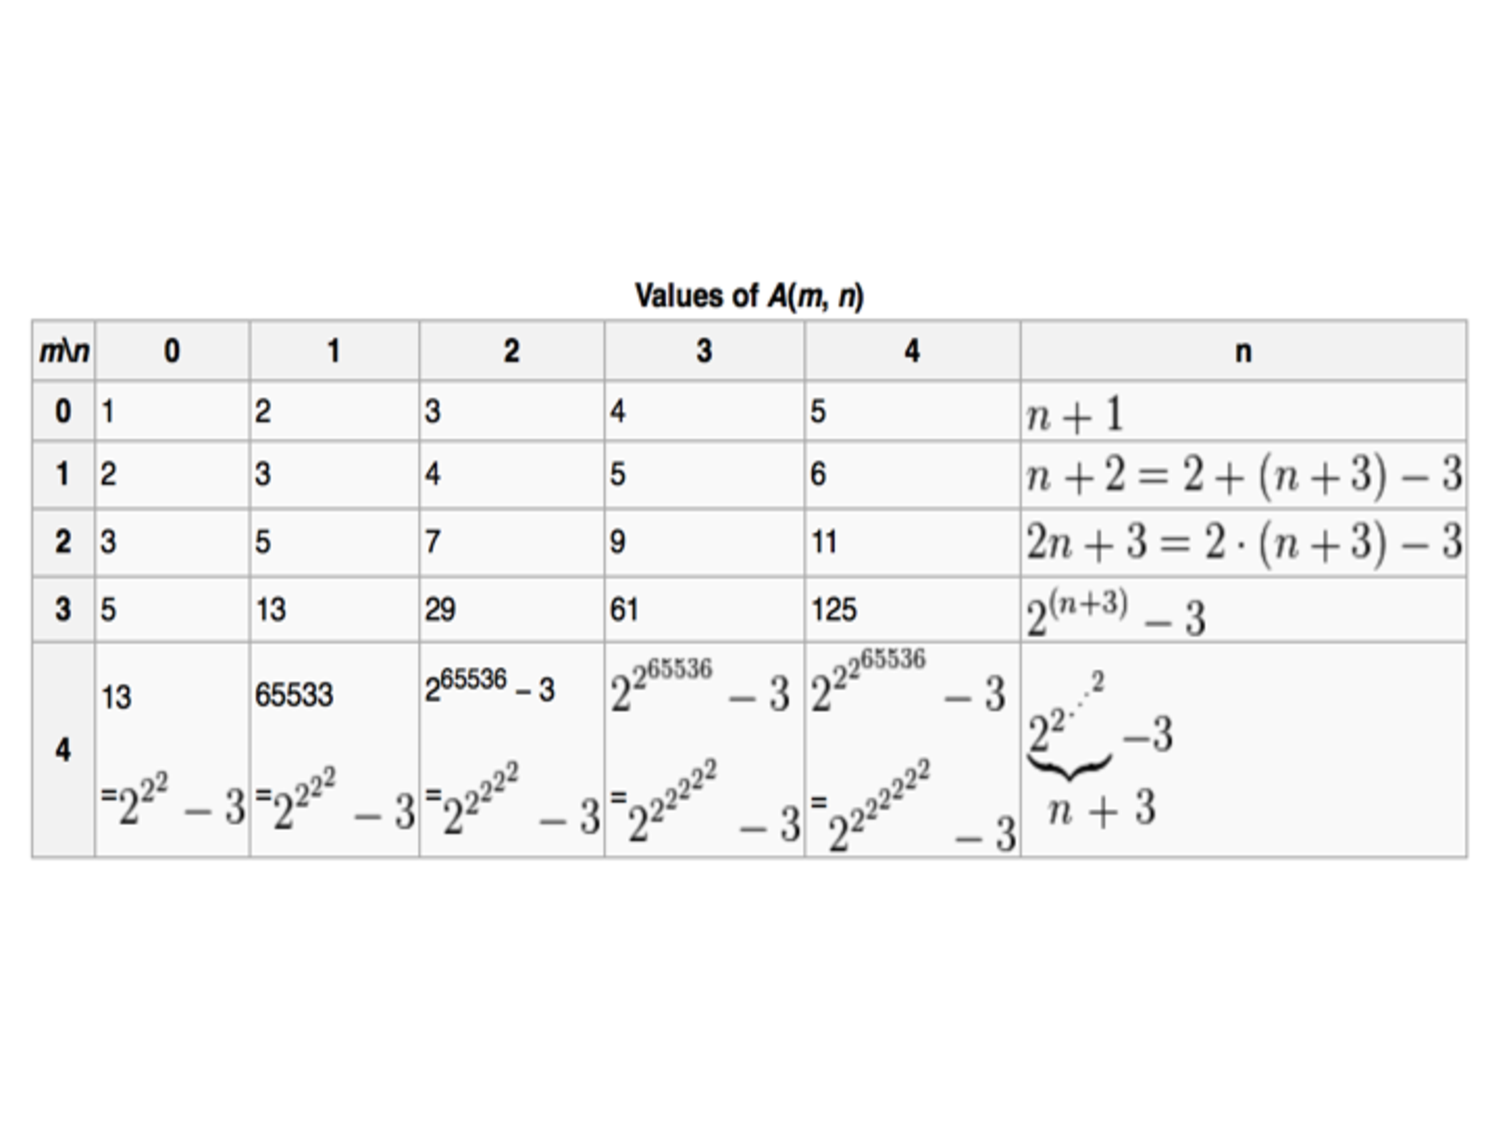
\includegraphics[scale=0.5]{img/ack}
\end{frame}


\begin{frame}[fragile]{Algoritmo de Euclides:Máximo divisor comum}
Alguns exemplos:
\begin{itemize}
 \item MDC(4,2) = ?
 \item MDC(8,7) = ?
 \item MDC(12,1) = ?
 \item MDC(20,15) = ?
 \item MDC(200,0) = ?
 \item MDC(X,Y) == MDC(Y,X) ?
\end{itemize}

\end{frame}

\begin{frame}{Algoritmo de Euclides}
Euclides achou um jeito bem legal de calcular (\blue{recursivamente}) o MDC
\begin{center}
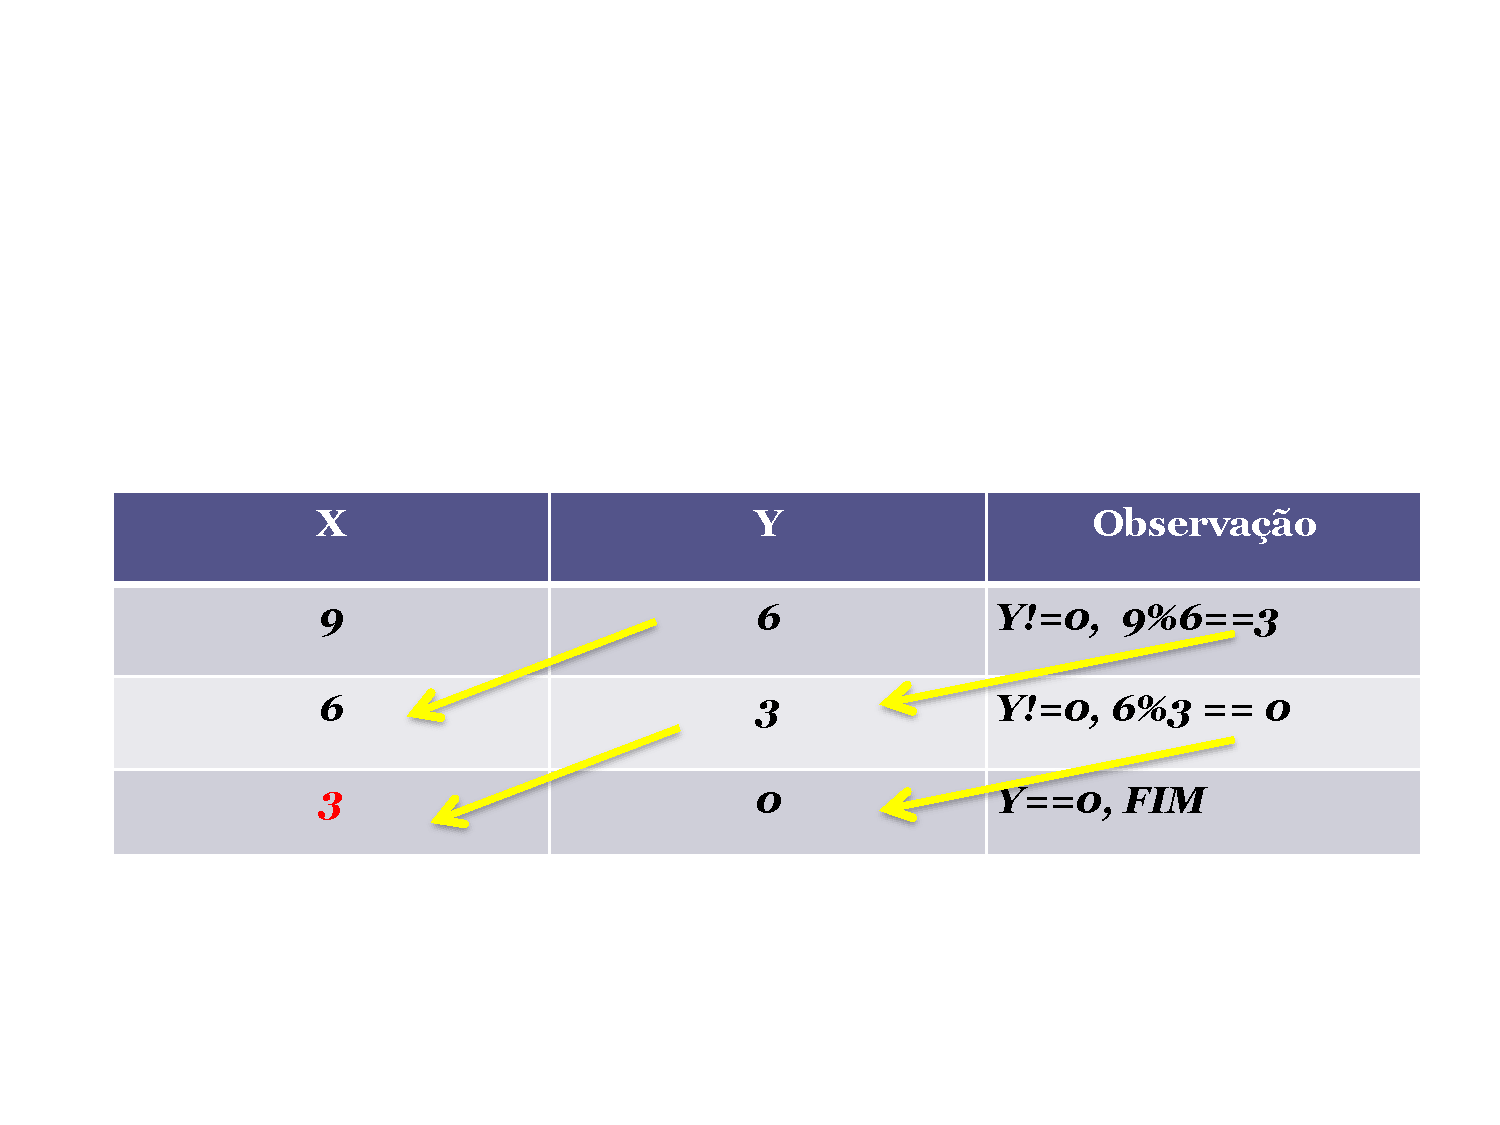
\includegraphics[scale=0.5]{img/euc}
\\
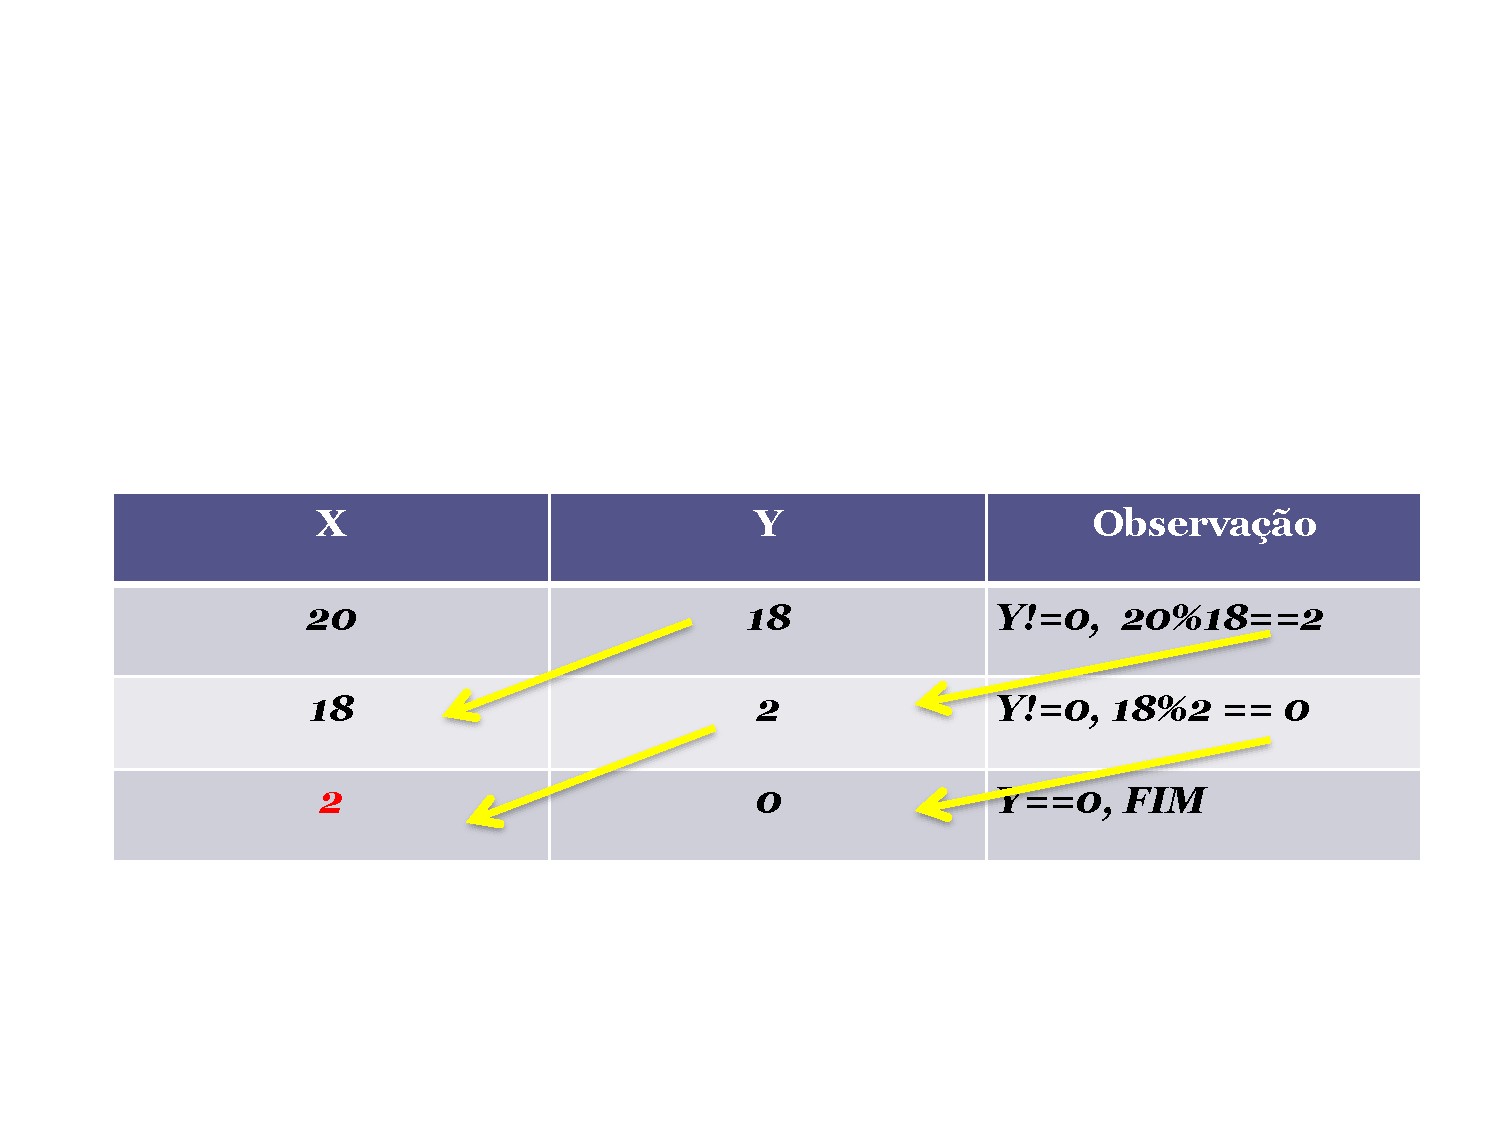
\includegraphics[scale=0.5]{img/euc2}
\end{center}
\end{frame}

\begin{frame}[fragile]{Algoritmo de Euclides}
\[
MDC(X,Y) = \left\{
\begin{array}{lll}
X & \quad & \mbox{ se  } Y = 0 \\
MDC(Y,X\%Y) & \quad & \mbox{ se  } Y > 0 \\
\end{array}
\right.
\]
\begin{lstlisting}
int euclides_MDC(int a, int b){
  if(b==0)
    return a;
  else
    return euclides_MDC(b,a%b);
}
\end{lstlisting}

\end{frame}

\begin{frame}{Busca em vetor ordenado}
\framesubtitle{Busca Binária}

\begin{itemize} 
 \item Faça uma função que dado um vetor de inteiros $v$ de tamanho $n$ e um número inteiro $x$, retorne o índice $m$ tal que $v[m]==x$. Se tal $m$ não existe, a função deve retornar  -1.

\end{itemize}

\begin{block}{}
Se o vetor $v$ está ordenado, nossa função poderia ser melhor ? 
\end{block}

\end{frame}


\begin{frame}{Exercícios}

Defina recursivamente as seguintes funções.  Assuma que os parâmetros $x$ e $y$ são inteiros positivos. 
\begin{itemize} 
 \item $mult:$    $x \times y$ (utilizando somas)
 \item $pow:$   $x^y$.  ( utilizando multiplicações) 
\end{itemize}

\begin{block}{Par / Ímpar}
Como poderia determinar se um inteiro positivo $x$ é par ou não sem utilizar o resto da divisão ? Dica. Defina uma função recursiva cujos casos base são:
\[
\begin{array}{lll}
\texttt{ehPar}(0) &\rightarrow &\texttt{true}\\
\texttt{ehPar}(1) &\rightarrow &\texttt{false}
\end{array}
\]
\end{block}
\end{frame}

\end{document}
